From \eqref{eq:conics/ex/solution/given} and \eqref{eq:conic_quad_form},
%
%\begin{align}
%\vec{x^T}\vec{V}\vec{x}+2\vec{u^T}\vec{x}+f=0\label{eq:conics/ex/solution/eqmain}
%\end{align}
%From the given second degree equation we get,
\begin{align}
\vec{V} &= \myvec{9&-12\\-12&16}\\ \label{eq:conics/ex/solution/given1}
\vec{u} &= \myvec{-9\\-\frac{101}{2}}\\ 
f &= 4 \label{eq:conics/ex/solution/given2}
\end{align}
\begin{enumerate}
\item Expanding the determinant of $\vec{V}$ we observe, 
\begin{align}
\mydet{9&-12\\-12&16} = 0 \label{eq:conics/ex/solution/eq2.1}
\end{align}
Also
\begin{align}
    \mydet{\vec{V} & \vec{u} \\ \vec{u}^T & f}=
    \mydet{9&-12 & -9 \\-12&16 & -\frac{101}{2} \\ -9 & -\frac{101}{2} & 4} \\
    \neq 0\label{eq:conics/ex/solution/eq2.2}
\end{align}
Hence from \eqref{eq:conics/ex/solution/eq2.1} and \eqref{eq:conics/ex/solution/eq2.2} we conclude that given equation is an parabola. The characteristic equation of $\vec{V}$ is given as follows,
\begin{align}
\mydet{\lambda\vec{I}-\vec{V}} = \mydet{\lambda-9&12\\12&\lambda-16} &= 0\\
\implies \lambda^2-25\lambda &= 0\label{eq:conics/ex/solution/eqchar}
\end{align}
Hence the characteristic equation of $\vec{V}$ is given by \eqref{eq:conics/ex/solution/eqchar}. The roots of \eqref{eq:conics/ex/solution/eqchar} i.e the eigenvalues are given by
\begin{align}
\lambda_1=0, \lambda_2=25\label{eq:conics/ex/solution/eqeigenvals}    
\end{align}
\item For $\lambda_1 = 0$, the eigen vector $\vec{p}$ is given by 
\begin{align}
\vec{V}\vec{p} = 0
%\\
%\brak{\lambda\vec{I}-\vec{V}}\vec{p}&=0 \label{eq:conics/ex/solution/eqev}
\end{align}
Row reducing $\vec{V}$ yields
\begin{align}
\implies
%\brak{\lambda_1\vec{I}-\vec{V}}&=
\myvec{-9&12\\12&-16}\xleftrightarrow[R_2=R_2+4R_1]{R_1=-\frac{R_1}{3}}\myvec{3&-4\\0&0}\\
\implies\vec{p}_1=\frac{1}{5}\myvec{-4\\-3} \label{eq:conics/ex/solution/eq2.3}
\end{align}
Similarly, 
\begin{align}
\vec{p}_2=\frac{1}{5}\myvec{-3\\4} 
%\label{eq:conics/ex/solution/eq2.3}
\end{align}
%
Thus, the eigenvector rotation matrix and the eigenvalue matrix are
%Substiuting equation \ref{eq:conics/ex/solution/eq2.3} in equation \ref{eq:conics/ex/solution/eqev} we get
%\begin{align}
%&\myvec{1&-\frac{4}{3}\\0&0}\myvec{v_1 \\ v_2}=\myvec{0 \\ 0}
%%\label{eq:conics/ex/solution/eqei1}
%\end{align}
%Where, $\vec{p}=\myvec{v_1\\v_2}$
%Let $v_2=t$
%\begin{align}
%    v_1&=\frac{4}{3}t
%\end{align}
%Eigen vector $\vec{p_1}$ is given by
%\begin{align}
%    \vec{p_1}&=\myvec{\frac{4}{3}t \\ t}
%\end{align}
%Let $t=-\frac{6}{10}$, we get
%\begin{align}
%        \vec{p_1}&=\myvec{-\frac{8}{10} \\-\frac{6}{10} }\label{eq:conics/ex/solution/eqp1}
%\end{align}
%Again, for $\lambda_2=25$,
%\begin{align}
%\brak{\lambda_2\vec{I}-\vec{V}}&=\myvec{16&12\\12&9}\xleftrightarrow[R_1=\frac{1}{16}R_1]{R_2=12R_1-R_2}\myvec{1&\frac{3}{4}\\0&0} \label{eq:conics/ex/solution/eq2.3.1}
%\end{align}
%Substiuting equation \ref{eq:conics/ex/solution/eq2.3.1} in equation \ref{eq:conics/ex/solution/eqev} we get
%\begin{align}
%&\myvec{1&\frac{3}{4}\\0&0}\myvec{v_1 \\ v_2}=\myvec{0 \\ 0}
%%\label{eq:conics/ex/solution/eqei1}
%\end{align}
%Where, $\vec{p}=\myvec{v_1\\v_2}$
%Let $v_2=t$
%\begin{align}
%    v_1&=-\frac{3}{4}t
%\end{align}
%Eigen vector $\vec{p_2}$ is given by
%\begin{align}
%    \vec{p_2}&=\myvec{-\frac{3}{4}t \\ t}
%\end{align}
%Let $t=-\frac{8}{10}$, we get
%\begin{align}
%        \vec{p_2}&=\myvec{\frac{6}{10} \\-\frac{8}{10} }
%%\label{eq:conics/ex/solution/eqp1}
%\end{align}
%The matrix $\vec{P}$,
\begin{align}
\vec{P}&=\myvec{\vec{p_1}&\vec{p_2}}=\frac{1}{5}\myvec{-4&-3\\ -3 &4} \\
\vec{D}&=\myvec{0&0\\0&25}
\end{align}
Table \ref{table:conics}, the focal length of the parabola is given by 
\begin{align}
\frac{\abs{2\vec{u}^T\vec{p_1}}}{\lambda_2}
    = \frac{75}{25}=3
\end{align}
%When $\mydet{\vec{V}}=0$,
%From 
%\eqref{eq:conics/ex/solution/eqmain} can be written as
and its equation is
\begin{align}
    \vec{y^T}\vec{D}\vec{y}&=-2\eta\myvec{1&0}\vec{y}\label{eq:conics/ex/solution/eq2.4}
\end{align}
where
\begin{align}
    \eta=\vec{u}^T\vec{p_1}=\frac{75}{2}
\end{align}
\begin{align}
    \myvec{\vec{u^T}+\eta\vec{p_1^T} \\ \vec{V}}\vec{c}=
    \myvec{-f \\ \eta\vec{p_1}-\vec{u}} 
\end{align}
using equations \eqref{eq:conics/ex/solution/given1},\eqref{eq:conics/ex/solution/given2} and \eqref{eq:conics/ex/solution/eq2.3}
\begin{align}
    \myvec{-39& -73 \\ 9 & -12 \\  -12 & 16 }\vec{c}=\myvec{-19 \\ -21\\ 28} \label{eq:conics/ex/solution/eqcen}
\end{align}
Forming the augmented matrix and row reducing it:
\begin{align}
\myvec{-39 & -73 & -19\\9 & -12 & -21 \\-12 & 16 &28 }\\
\xleftrightarrow[]{R_3\leftarrow R_3+(4/3)R_2} 
\myvec{-39 & -73 & -19\\9 & -12 & -21 \\0 & 0 &0 }\\
\xleftrightarrow[]{R_1\leftarrow R_1/(-39)} 
\myvec{1 & 73/39 & 19/39\\9 & -12 & -21 \\0 & 0 &0 }\\
\xleftrightarrow[]{R_2\leftarrow R_2-9R_1}
\myvec{1 & 73/39 & 19/39\\0 & -1125/39 & -990/39 \\0 & 0 &0}\\ 
\xleftrightarrow[]{R_2\leftarrow R_2 \times (-39/1125)}
\myvec{1 & 73/39 & 19/39\\0 & 1 & 22/25 \\0 & 0 &0}\\
\xleftrightarrow[]{R_1\leftarrow R_1 -(73/39)R_2}
\myvec{1 & 0 & -29/25\\0 & 1 & 22/25 \\0 & 0 &0}
\end{align}
Thus the vertex $\vec{c}$ is:
\begin{align}
\vec{c}=\myvec{ -29/25\\22/25}= \myvec{-1.16\\ 0.88} 
\end{align}

%and the vertex $\vec{c}$ is given by 
%\begin{align}
%    \myvec{\vec{u^T}+\eta\vec{p_1^T} \\ \vec{V}}\vec{c}=
%    \myvec{-f \\ \eta\vec{p_1}-\vec{u}} 
%\end{align}
%using equations \eqref{eq:conics/ex/solution/given1},\eqref{eq:conics/ex/solution/given2} and \eqref{eq:conics/ex/solution/eq2.3}
%\begin{align}
%    \myvec{-69& -\frac{191}{2} \\ 9 & -12 \\  -12 & 16 }\vec{c}=\myvec{-4 \\ -51 \\ \frac{11}{2}} \label{eq:conics/ex/solution/eqcen}
%\end{align}
% This is in the form of 
% \begin{align}
% {A}\vec{c}=\vec{b}
% \end{align}
%  \begin{align} 
% \intertext{using least squares solution of linear system}
% {A}^T{A}\vec{c}={A}^T\vec{b}
% \implies \vec{c}=  ({{A}^T{A}})^{-1} {A}^T\vec{b} \label{eq:conics/ex/solution/main}
%\end{align}
%\begin{align}
%{A}^T{A}=\myvec{-69 & 9 & -12 \\ -\frac{191}{2}& -12& 16 }
% \myvec{-69& -\frac{191}{2} \\ 9 & -12 \\  -12 & 16 } \nonumber \\ \implies
% {A}^T{A}=\myvec{4986& \frac{12579}{2} \\  \frac{12579}{2} & \frac{38081}{4} }
%\end{align}
%The inverse can be written as
%\begin{align}
%    ({{A}^T{A}})^{-1}=\frac{31640625}{4}
%    \myvec{\frac{38081}{4}&- \frac{12579}{2} \\  -\frac{12579}{2} & 4986}\label{eq:conics/ex/solution/con1}
%\end{align} 
%\begin{align}
%   {A}^T\vec{b} = \myvec{-69 & 9 & -12 \\ -\frac{191}{2}& -12& 16 }\myvec{-4 \\ -51 \\ \frac{11}{2}} \nonumber \\
%   {A}^T\vec{b} =\myvec{-249 \\ 1082} \label{eq:conics/ex/solution/con2}
%\end{align}
%using \ref{eq:conics/ex/solution/con1} and \ref{eq:conics/ex/solution/con2} in \ref{eq:conics/ex/solution/main},the center $\vec{c}$
%\begin{align}
%    \vec{c}=\frac{31640625}{4}
%    \myvec{\frac{38081}{4}&- \frac{12579}{2} \\  -\frac{12579}{2} & 4986}\myvec{-249 \\ 1082} \\
%    \implies \vec{c}=\myvec{-\frac{29}{25} \\ \frac{22}{25}} 
%\end{align}

\begin{figure}[!ht]
    \centering
    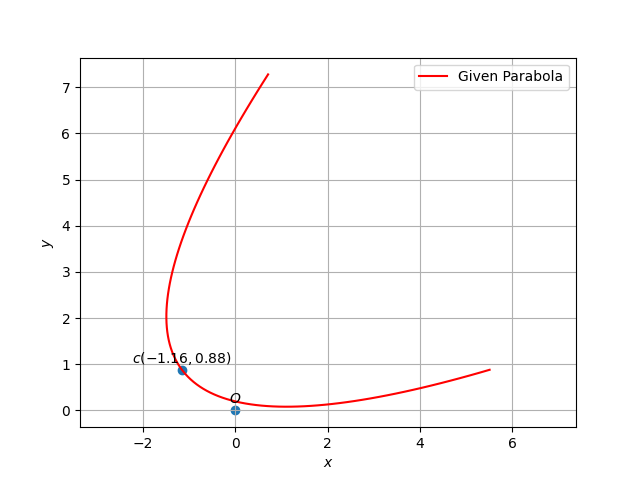
\includegraphics[width=\columnwidth]{./figs/parab/parab_gen.png}
    \caption{Parabola with the center c}
    \label{eq:conics/ex/solution/Fig:1}
\end{figure}
\end{enumerate}
